%
\documentclass{beamer}
%%\documentclass[handout]{beamer}

\definecolor{headcolor}{rgb}{0,0.3,0.6}
%\renewcommand{\alert}[1]{\textcolor{headcolor}{#1}}
\renewcommand{\alert}[1]{\textcolor{blue}{#1}}
\newcommand{\red}[1]{\textcolor{red}{#1}}
\mode<presentation>
{
  \usetheme{default}
  %% \setbeamercovered{transparent}
  \usefonttheme{professionalfonts}
  \usefonttheme{structurebold}
  \usecolortheme[rgb={0,0.3,0.6}]{structure}
  %%  \usecolortheme[rgb={0,0,0.7}]{structure}
}

\usepackage[english]{babel}
\usepackage[latin1]{inputenc}
\usepackage{times}
\usepackage[T1]{fontenc}
\usepackage{rotate}
\usepackage{color}
\usepackage{verbatim}
\usepackage{xmpmulti}
\usepackage{pgfarrows}
%\usepackage{pgf}

%\input{/home/tom/lib/tex/defs}
%%%%%%%%%%%%%%%%%%%%%%%%%%%%%%%%%%%%

% Delete this, if you do not want the table of contents to pop up at
% the beginning of each subsection:
%\AtBeginSection[]
%{
%  \begin{frame}<beamer>
%    \frametitle{Outline}
%    \tableofcontents[currentsection]
%  \end{frame}
%}
% \AtBeginSubsection[]
% {
%   \begin{frame}<beamer>
%     \frametitle{Outline}
%     \tableofcontents[currentsubsection]
%   \end{frame}
% }

% If you wish to uncover everything in a step-wise fashion, uncomment
% the following command: 
%\beamerdefaultoverlayspecification{<+->}

%%%%%%%%%%%%%%%%%%%%%%%%%%%%%%%%%%%%%%%%%%%%%%%%%%%%%%%%%%%%%%%%%%%%%%%%%%%%%%%

\def\width{12.5} % slide width
\def\height{8.5} % slide height
\newcommand{\showgrid}{%
  \pgfsetlinewidth{0.8pt} 
  \pgfgrid[step={\pgfpoint{1cm}{1cm}}]{\pgforigin}{\pgfxy(\width,\height)}{} 
  \pgfsetlinewidth{0.1pt} 
  \pgfgrid[stepx=0.1cm,stepy=0.1cm]{\pgforigin}{\pgfxy(\width,\height)}
}
\newcommand{\pgfslide}[1]{%
  \hspace*{-1cm}
  \begin{pgfpicture}{0cm}{0cm}{\width cm}{\height cm}
    #1
  \end{pgfpicture}  
}
\def\figpath{figs/}


%%%%%%%%%%%%%%%%%%%%%%%%%%%%%%%%%%%%
\newcommand{\A}{{\text{A}^{-}}}
\newcommand{\Ca}{{\text{Ca}^{2+}}}
\newcommand{\Cl}{{\text{Cl}^{-}}}
\newcommand{\di}{\text{d}}
\newcommand{\diff}[2]{\displaystyle\frac{\text{d}#1}{\text{d}#2}}
\newcommand{\e}{\text{e}}
\newcommand{\Epop}{\mathcal{E}}
\newcommand{\EW}[2][]{\text{E}_{#1}\left[#2\right]}
\newcommand{\Ex}{\text{E}}
\newcommand{\FT}{\mathfrak{F}}
\newcommand{\iFT}{\mathfrak{F}^{-1}}
\newcommand{\Fourier}[2]{\mathfrak{F}\left[#1\right]\left(#2\right)}
\newcommand{\iFourier}[2]{\mathfrak{F}^{-1}\left[#1\right]\left(#2\right)}
\newcommand{\In}{\text{I}}
\newcommand{\inp}{\text{inp}}
\newcommand{\Ipop}{\mathcal{I}}
\newcommand{\K}{{\text{K}^{+}}}
\newcommand{\Leak}{{\text{L}}}
\newcommand{\mm}{\text{mm}}
\newcommand{\mV}{\text{mV}}
\newcommand{\Na}{{\text{Na}^{+}}}
\newcommand{\one}{\mathbb{I}}
\newcommand{\rest}{\text{rest}}
\newcommand{\tauM}{\tau_\text{m}}
\newcommand{\tauR}{\tau_\text{ref}}
\newcommand{\vect}[2]{\begin{pmatrix}#1\\#2\end{pmatrix}}
%%%%%%%%%%%%%%%%%%%%%%%%%%%%%%%%%%%%

%%%%%%%%%%%%%%%%%%%%%%%%%%%%%%%%%%%%%%%%%%%%%%%%%%%%%%%%%%%%%%%%%%%%%%%%%%%%%%%
\begin{document}
%%
%% title page
\begin{frame}
  \pdfbookmark[2]{Title}{TitlePage}
  \pgfslide{
    %% 
    \pgfputat{\pgfxy(6.25,8)}{\pgfbox[center,top]{\parbox{12.5cm}{\centering
          \LARGE\color{headcolor}{
            %%
            {\bfseries Simulation of Biological Neuronal Networks}\\[0.3cm]
            %%
            {Neuron Models}\\
            %% 
          }
        }}}
    %% 
    \pgfputat{\pgfxy(6.25,4.0)}{\pgfbox[center,top]{\parbox{12.5cm}{\centering
          {\large Robin Pauli, Abigail Morrison}\\[0.2cm]
          {\small{} \{r.pauli\textbar morrison\}@fz-juelich.de{}}
        }}}
        
    %%
    \pgfputat{\pgfxy(6.25,2.0)}{\pgfbox[center,top]{\parbox{12.5cm}{\centering
          \footnotesize
          Inst.~of Neuroscience and Medicine (INM-6)\\
          Computational and Systems Neuroscience\\
          Research Center J\"ulich, Germany
        }}}
    %%
    \pgfputat{\pgfxy(0.5,-0.7)}{\pgfbox[left,bottom]{\parbox{12.5cm}{
          \footnotesize 
some time July        }}}
    %% \showgrid
  }
\end{frame}
%%%%%%%%%%%%%%%%%%%%%%%%%%%%%%%%%%%%%%%%%%%%%%%%%%%%%%%%%%%%%%%%%%%%%%%%%%%

%%%%%%%%%%%%%%%%%%%%%%%%%%%%%%%%%%%%%%%%%%%%%%%%%%%%%%%%%%%%%%%%%%%%%%%%%%%


%%%%%%%%%%%%%%%%%%%%%%%%%%%%%%%%%%%%%%%%%%%%%%%%%%%%%%%%%%%%%%%%%%%%%%%%%%%
%\section{\ttl}
\begin{frame}
  \frametitle{The Neuron}
  All Neurons share key features:
  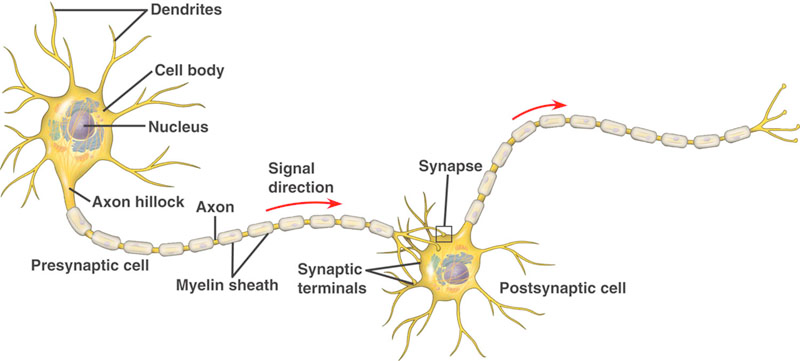
\includegraphics[width=\textwidth]{fig/neuronscheme.png}
  \begin{itemize}
  \item input: dendrites ("belonging to the tree")
  \item integration: soma ("cell body")
  \item long range conduction: axon ("axis")
  \item output: synapse ("conjunction") 
  \end{itemize}
\end{frame}
%%%%%%%%%%%%%%%%%%%%%%%%%%%%%%%%%%%%%%%%%%%%%%%%%%%%%%%%%%%%%%%%%%%%%%%%%%%

\begin{frame}
\frametitle{Outline}
\begin{itemize}
\item Review of spatial structure and dynamics of a     physiological neuron
\item  Modeling approaches: detail or abstraction?
\item  Representation of physiological neuron features in   a point neuron model
\item  Advantages of the point neuron modeling approach
\item  Simulating a mathematical model
\item  Choosing a model

\end{itemize}

\end{frame}

\begin{frame}
\frametitle{Spatial Structure}
\begin{itemize}
\item There uncountable different neuron types
\end{itemize}
\includegraphics[width = 0.9\textwidth]{fig/{neuron_types}.png}\\
{\tiny based on drawings by Ramon y Cajal 1852-1934}
\end{frame}

\begin{frame}
\frametitle{Resting Potential}
\begin{columns}
\column{0.55\textwidth}
\flushleft

\begin{itemize}
\only<1>{
\item neuron have a voltage called resting potential
\item determined by concentration gradients and membrane permeability
\item active Ion pumps move 3 $\text{Na}^+$, 2 $\text{K}^+$ Ions to keep up gradients\\
\item Nernst Potential: $E_{eq,K^+} = \frac{RT}{zF} \ln \frac{[K^+]_{o}}{[K^+]_{i}}  = 61.54 mV \log \frac{[K^+]_{o}}{[K^+]_{i}}$
\item $E_{m} = \frac{g_{K^+}E_{eq,K^+} + g_{Na^+}E_{eq,Na^+} + g_{Cl^-}E_{eq,Cl^-}} {g_{K^+}+g_{Na^+}+g_{Cl^-}}$
}
\only<2>{
\item In response to depolarization: $Na^+$ open, $K^+$ still closed
\item At peak Action potential: $Na^+$ close, $K^+$ open
\item Hyperpolarization: $K^+$ leads to overshoot
}
\only<2>{
\flushleft
\vspace{-.7cm}
\includegraphics[width=0.9\textwidth]{fig/{AP}.png}
}
\end{itemize}

\column{0.5\textwidth}\flushright\hfill
\vspace{-1.5cm}
\includegraphics[width=1.0\textwidth]{fig/{restingpotential_AP}.jpeg}
\end{columns}

\end{frame}


\begin{frame}
\frametitle{Essential features of neurons}

\begin{itemize}
\item Connectivity/morphology
\item Internal dynamics that integrate inputs
\item generation of action potentials
\end{itemize}
If we want to investigate these features outside of experiments
 we need to captures these features\\

Two main approaches
\begin{itemize}
\item detailed (biophysical) neuron models
\item Reduced (abstract) neuron models
\end{itemize}
we will focus on the latter one specifically point neuron models

\end{frame}


\begin{frame}
\frametitle{Detailed neuron models}
\begin{columns}
\column{0.5\textwidth}
\includegraphics[width=1.0\textwidth]{fig/{mcn}.png}
\column{0.5\textwidth}\flushright\hfill
\includegraphics[width=1.1\textwidth]{fig/{mcmabstract}.png}
\begin{itemize}
\item Reconstruct neuron morphology from images
\item decompose into compartments (between branches)
\item define/fit/tune properties of individual compartments
\item Simulate in e.g. Neuron
\end{itemize}
\end{columns}
\end{frame}

\begin{frame}
\frametitle{Detailed neuron models}
Morphology is reduced to a directed graph:
\includegraphics[width=1.0\textwidth]{fig/{adjacency}.png}\\
(or any network)\\
Connectivity matrix can be updated to include connection weight
\end{frame}


\begin{frame}
\frametitle{Why all this complexity?}
\includegraphics[height=0.8\textheight]{fig/{dendspike}.png}\\
Some effects like dendritic spikes or backpropagation need morphology
\end{frame}

\begin{frame}
\frametitle{Point Neuron Models: dynamics}
\begin{itemize}
\item 
Membrane potential is driven by external and ionic current:\\
$I_{e} = C_m\frac{{\mathrm d} V_m}{{\mathrm d} t}+I_{c}$
\item Current is determined by Ion flow through channels:\\
\item $I_{c}= - \bar{g}_\text{K}n^4(V_m - V_K) - \bar{g}_\text{Na}m^3h(V_m - V_{Na}) - \bar{g}_l(V_m - V_l),$
\begin{enumerate}
\item $\frac{dn}{dt} = \alpha_n(V_m)(1 - n) - \beta_n(V_m) n$
\item $\frac{dm}{dt} = \alpha_m(V_m)(1 - m)  - \beta_m(V_m) m$
\item $\frac{dh}{dt} = \alpha_h(V_m)(1 - h) - \beta_h(V_m) h$
\end{enumerate}

\end{itemize}
\centering
\includegraphics[height=0.5\textheight]{fig/{HH}.png}\\

\end{frame}

\begin{frame}
\frametitle{Point Neuron Models: dynamics}
\begin{columns}
\column{0.5\textwidth}
\begin{itemize}
\item 
From Kirchhoff's law:\\
$C_m\frac{{\mathrm d} V_m}{{\mathrm d} t} =\frac{V_m}{R}+I_{ext}$
\item Threshold behaviour\\
$V_m > \Theta \rightarrow V_m=V_{rest}$
\end{itemize}
\column{0.5\textwidth}
Additional simplifications:

\begin{itemize}
\item linear subthreshold integration
\item time invariant parameters
\end{itemize}
\end{columns}


\includegraphics[width=1.\textwidth]{fig/{iaf}.jpg}\\

\end{frame}

\begin{frame}
\frametitle{Synaptic transmission: COBA vs. CUBA}

\begin{columns}
\column{0.5\textwidth}
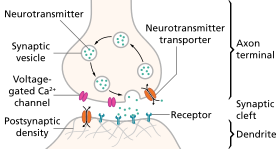
\includegraphics[width=\textwidth]{fig/SynapseSchematic.png}\\
\begin{itemize}
\item COBA i.e. change in conductace
\item CUBA i.e. current flow irrespective of membrane potential
\item can be positive (glutamate) or negative (GABA)\\

\end{itemize}
\column{0.5\textwidth}
\begin{itemize}
\item Ionotropic or metabotropic,
\item Ionotropic: ion channel is activated
\item Metabotropic:\\
 activates G-protein,\\
  activates secondary messenger,\\
   which activates something else
\item may or may not result in current flow,\\
 can also change synaptic plasticity
\end{itemize}
\end{columns}



\end{frame}

\begin{frame}
\frametitle{Comparing Detailed vs. abstract}
\begin{itemize}
\item Detailed neuron models:
\begin{itemize}

 \item Have physical extent
 \item Give a good approximation of the electrical properties of a physiological neuron
 \item Can be made arbitrarily complex
\end{itemize} 

\item Point neuron models:
\begin{itemize}

 \item Have no physical extent
 \item Represent the dynamics in an extremely reduced fashion
 \item Are very simple
\end{itemize} 
\end{itemize}
{\huge Why would anyone want to use a point neuron model?}

\end{frame}


\begin{frame}
\frametitle{Comparing Detailed vs. abstract}
\begin{itemize}
\item Much less initial investment
\item Analysis, some models might be analytically tractable
\item Network simulation
\item Not as bad an approximation as one might think
\end{itemize}


\end{frame}

\begin{frame}
\frametitle{Not that bad}
\includegraphics[width=1.\textwidth]{fig/{kobayashi_neuron}.jpg}\\

Kobayashi et al. 2009, Izhikevic 2004
\end{frame}

\begin{frame}
\frametitle{Not that bad}
\includegraphics[width=1.\textwidth]{fig/{challenge}.png}\\

\end{frame}

\begin{frame}
\frametitle{Not that bad}
\begin{columns}
\column{0.5\textwidth}
\visible<1->{

\includegraphics[width=1.\textwidth]{fig/{kobayashi_price}.png}\\}

\column{0.5\textwidth}
\visible<2>{
\includegraphics[width=1.\textwidth]{fig/{kobayashi_PRICE}.png}\\}

\end{columns}
\visible<1->{
\center
\includegraphics[height=.4\textheight]{fig/{challenge}.png}\\}

\end{frame}


\begin{frame}
\frametitle{Not that bad}
\begin{itemize}
\item Point neurons won all challenges in all years, despite behaviorally relevant incentives

\item The MAT2 model (Kobayashi et al., 2009) only has one dynamic variable more than the standard leaky IaF model
\item 
The arbitrary complexity of biophysical neuron models makes them a parameter fitting nightmare
\item Save complexity for when you really need it

\end{itemize}

\end{frame}

\end{document}


%%
%% template
%%%%%%%%%%%%%%%%%%%%%%%%%%%%%%%%%%%%%%%%%%%%%%%%%%%%%%%%%%%%%%%%%%%%%%%%%%%
\def\ttl{}
\section{\ttl}
\begin{frame}
  \frametitle{\ttl}
  \pgfslide{
  %%
  %%
  %%\showgrid
  }
\end{frame}
%%%%%%%%%%%%%%%%%%%%%%%%%%%%%%%%%%%%%%%%%%%%%%%%%%%%%%%%%%%%%%%%%%%%%%%%%%%


